% Auteur : Romain TESTUD
\begin{frame}{Le protocole Wormhole}
    \begin{block}{Mise en contexte}
        \begin{itemize}
            \item Solution d'échanges inter-blockchains.
            \item utilisation de bridges.
        \end{itemize}
    \end{block}
    \begin{block}{Les étapes d'un transfert}
        \begin{itemize}
            \item Formulation de la transaction.
            \item Récupération et vérification des signatures des gardiens.
            \item Envoi de la transaction.
        \end{itemize}
    \end{block}
    \begin{figure}
        \centering
        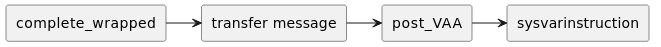
\includegraphics[scale = 0.3]{centralisation/img/fonctions.png}
        \caption{Fonctions appelées lors d'un transfert}
    \end{figure}
\end{frame}

\begin{frame}{L'attaque}
    \begin{block}{Attaque sur le bridge entre Solana et Ethereum}
        \begin{itemize}
            \item Le 2 Février 2022.
            \item 120 000 ETH de perte.
            \item Correction de bug publié mais pas encore en production.
        \end{itemize}
    \end{block}
\end{frame}

\begin{frame}{L'attaque}
    \begin{block}{Passer la signature des gardiens?}
        Utilisation de signatures d'une transaction antérieure.
    \end{block}
    \begin{block}{Passer la vérification ?}
        \begin{itemize}
            \item Exploitation d'une erreur d'implémentation dans \textit{verify\_signature}
            \item Appel à un programme externe.
        \end{itemize}
        \begin{figure}
            \centering
            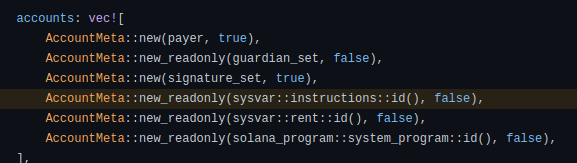
\includegraphics[scale = 0.3]{centralisation/img/sysvar_atk.png}
            \caption{Appel à la fonction de vérification}
        \end{figure}
    \end{block}
\end{frame}

\begin{frame}{L'attaque}
    \begin{itemize}
        \item Utilisation d'une nouvelle adresse.
        \item Validation des signatures par défaut.
    \end{itemize}
    \begin{figure}
        \centering
        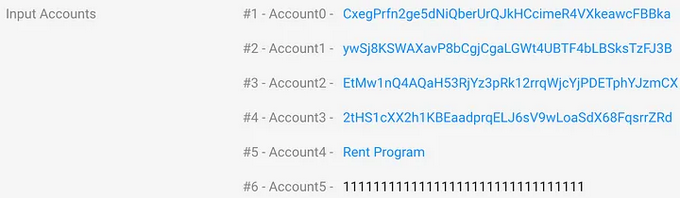
\includegraphics[scale = 0.3]{centralisation/img/sysvar_transaction.png}
        \caption{Appel à la fonction de vérification}
    \end{figure}
\end{frame}

\begin{frame}
    \begin{block}{Transaction validée et envoyée}
        \begin{itemize}
            \item 120 000 ETH transmis.
            \item Sans avoir déposé de jetons au préalable.
        \end{itemize}
    \end{block}
\end{frame}

\begin{frame}{Correctif}
    \begin{itemize}
        \item Vérification de l'appel par \textit{sysvar\_instruction}
    \end{itemize}
    \begin{figure}
        \centering
        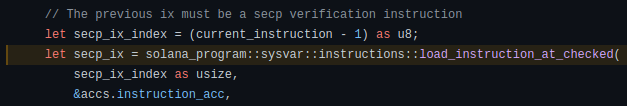
\includegraphics[scale = 0.3]{centralisation/img/worm_fixed.png}
        \caption{Appel à la fonction de vérification}
    \end{figure}
\end{frame}